\section{Eksperymenty}
Teraz chciałbym pokazać jak działa moja aplikacja. W tym celu spróbuję trochę poeksperymentować z danymi i pokazać to, co do tej pory udało się osiągnąć.


Wyobraźmy sobie sytuację że robimy system rejestrujący badania medyczne wykonane na rzecz pacjenta. Chcielibyśmy się dowiedzieć, czy rejestrowane badanie jest badaniem refundowanym (nasza wyobrażona refundacja dotyczy tylko badań zarejestrowanych w roku 2019). O czasie rejestracji badania mówi zmienna ,,data\_rejestracji\_badania''. W przypadku gdy badanie nie jest refundowane system ma wyświetlić komunikat informacyjny. 

Na początek definicja reguły, niech brzmi ona następująco:
\\ \\
\fbox{\begin{minipage}{40em}
\textit{Jeżeli data\_rejestracji\_badania jest mniejsza niż '01-01-2019' wtedy wyświetl komunikat "Badanie sprzed okresu refundacji".}
\end{minipage}}
\\ \\
Wprowadzam ją do systemu, i wygląda to tak:
\begin{figure}[H]
	\centering
	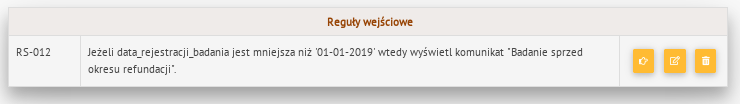
\includegraphics[scale=0.8]{img/app-eksperymenty/p1-1.png}
\end{figure}

\newpage
Teraz spójrzmy czego udało się o niej dowiedzieć:
\begin{figure}[H]
	\centering
	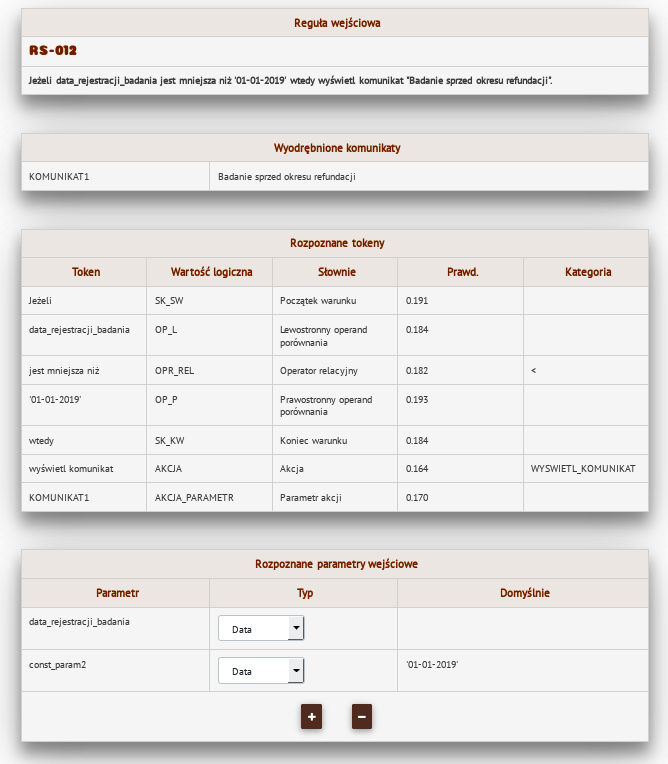
\includegraphics[scale=0.9]{img/app-eksperymenty/p1-2.png}
\end{figure}

\begin{itemize}
	\item \textbf{Reguła wejściowa} - system jeszcze raz przypomina treść wprowadzonej reguły i prezentuje nadany jej kod, w naszym przypadku RS-012.
	\item \textbf{Wyodrębnione komunikaty} - tu zaprezentowane zostały komunikaty, które udało się wyszukać w regule. Każdy odnaleziony komunikat zostaje wycięty z reguły przed poddaniem jej analizie i zastąpiony swoim reprezentującym go identyfikatorem - w naszym przypadku odnaleziony został jeden komunikat i zastąpiony przez słowo \textit{,,KOMUNIKAT1''}.
	\item \textbf{Rozpoznane tokeny} - najistotniejsza część wyników analizy. Widzimy, że z tą regułą algorytm poradził sobie bezbłędnie. Tokeny zostały prawidłowo skojarzone z ich znaczeniem logicznym. \\
	Na chwilę uwagi zasługuje tylko kolumna ,,Kategoria'' . Dotyczy ona tych tokenów, które mogą być określone na wiele sposobów. Musimy przyporządkować im jedną, uniwersalną kategorię. Jako przykład niech posłuży operator mniejszości - może on zostać opisany jako (,,jest mniejszy niż'',,,jest mniejszy od'',,,jest mniejsza od'',\dots). Z punktu widzenia aplikacji, wszystkie te wartości reprezentują jedną kategorią, ja nazwałem ją po prostu ,,<'' .
	\item {Rozpoznane parametry wejściowe} - w tym miejscu pokazywane są wartości, które uznane zostały za parametry wejściowe reguły. Trafiają tu tokeny, które biorą udział w porównaniach, lub są przekazywane jako parametry wejściowe do innych reguł (tę sytuację pokażę trochę później). W tym przypadku widzimy, że aplikacji udało się prawidłowo dopasować typy danych i określić wartość domyślną jednego z parametrów. Gdyby to się nie udało, czynność tę musi wykonać człowiek. Musi się to stać przed wygenerowaniem kodu.
\end{itemize}


I na koniec spójrzmy na wygenerowany kod metody walidującej regułę RS-012.
\begin{figure}[H]
	\centering
	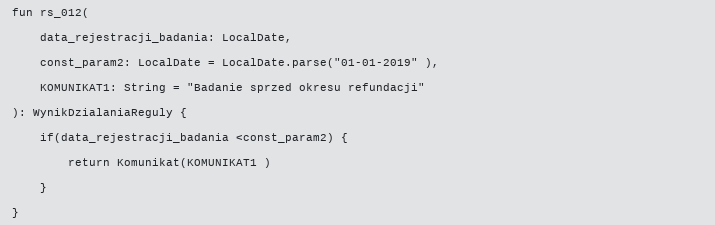
\includegraphics[scale=0.8]{img/app-eksperymenty/p1-3.png}
\end{figure}

Wszystko wygląda ok, więc spróbujmy trochę skomplikować regułę. 

\paragraph{}
Załóżmy że refundacji podlegają tylko te badania, które zostały wykonane w pierwszym kwartale 2019 roku. Chcielibyśmy zmienić treść reguły w taki sposób, by po stwierdzeniu tego typu sytuacji informowała użytkownika że jego badanie może zostać zrefundowane.
\\ \\
\fbox{\begin{minipage}{40em}
		\textit{Jeżeli data\_rejestracji\_badania jest mniejsza niż '01-01-2019' lub data\_rejestracji\_badania nie jest większa niż '01-04-2019' wtedy wyświetl komunikat "Badanie sprzed okresu refundacji".}
\end{minipage}}
\\ \\
Modyfikuję regułę:
\begin{figure}[H]
	\centering
	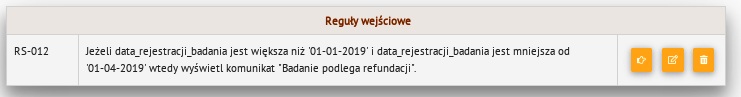
\includegraphics[scale=0.8]{img/app-eksperymenty/p2-1.png}
\end{figure}
I oglądamy wyniki:
\begin{figure}[H]
	\centering
	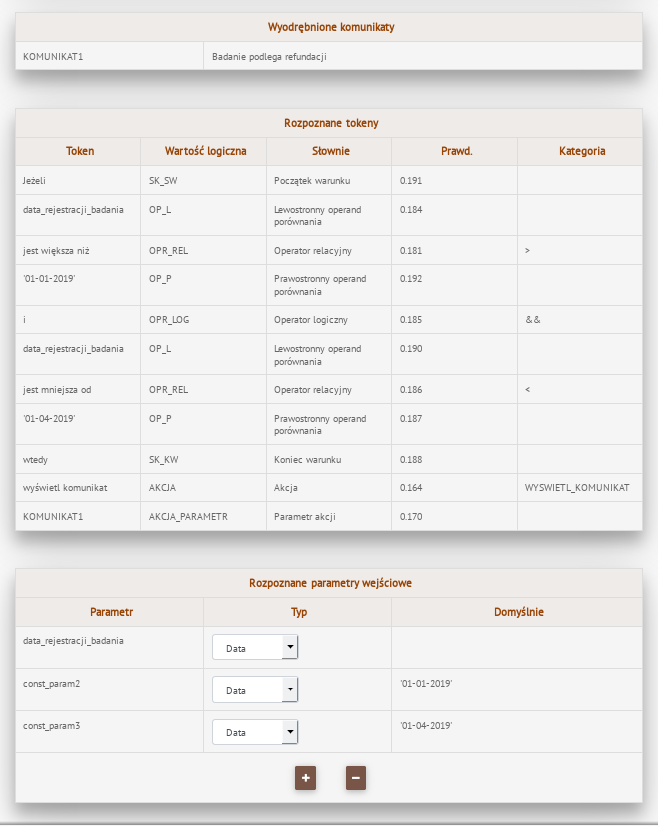
\includegraphics[scale=0.8]{img/app-eksperymenty/p2-2.png}
\end{figure}
Istotne zmiany doszły w tabeli rozpoznanych tokenów. Doszedł operator logiczny, oraz druga część warunku. Udało się również prawidłowo przyporządkować operatory do określających je kategorii. Dodatkowo doszedł nowy parametr wejściowy, którego zadaniem jest definiować drugą porównywaną wartość. 

Wygenerowany kod również wygląda na poprawny:
\begin{figure}[H]
	\centering
	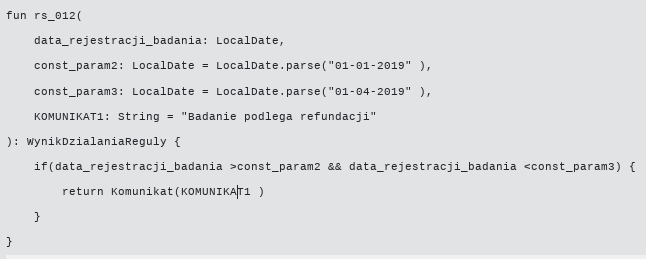
\includegraphics[scale=0.8]{img/app-eksperymenty/p2-3.png}
\end{figure}

Ponownie zmodyfikujmy regułę:
\begin{figure}[H]
	\centering
	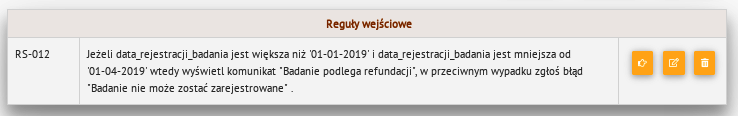
\includegraphics[scale=0.8]{img/app-eksperymenty/p3-1.png}
\end{figure}

\begin{figure}[H]
	\centering
	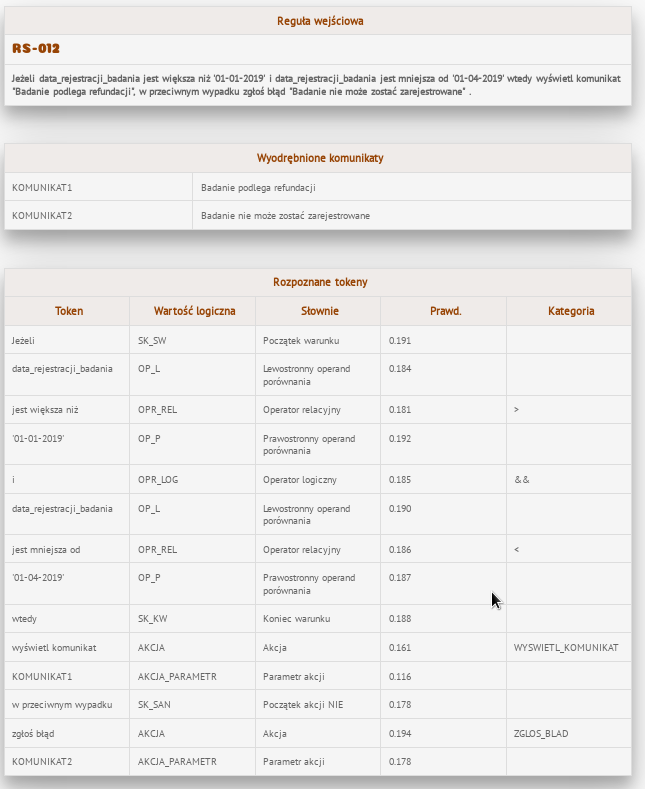
\includegraphics[scale=0.8]{img/app-eksperymenty/p3-2.png}
\end{figure}

\begin{figure}[H]
	\centering
	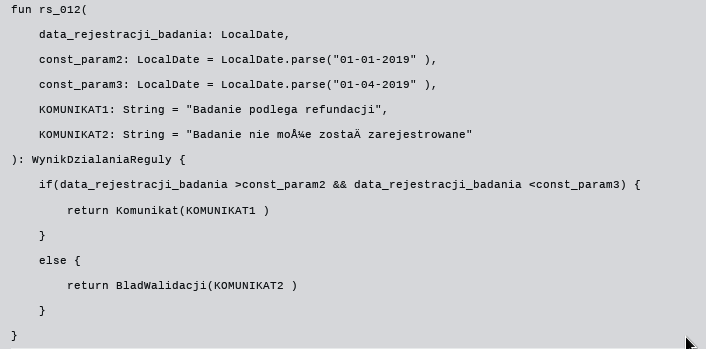
\includegraphics[scale=0.8]{img/app-eksperymenty/p3-3.png}
\end{figure}